\chapter{Real-data studies and interpretation}
\label{ch:realdata}\label{sec:realdata}
\chapterpromise{Four real executed fits, their exact data and model semantics, comparator limits, and two immutable computations excluded from incompatible scientific interpretations.}

\section{Interpretation policy}
The four case studies are real executed BayesBreak fits with archived data hashes and four-of-four
DP diagnostic checks. Red vertical lines in the current figures are fitted MAP boundaries unless an
independent annotation source is explicitly identified; they are not treated as geology, macro-event,
copy-number, or atlas ground truth. Panel~D in each generic case-study figure is an in-sample
cumulative diagnostic, not held-out evaluation.

\subsection{Well-log NMR response}
\label{sec:realdata-welllog}
The archived source describes the O Ruanaidh well-log NMR response with 4,050 original values and an
executed downsampled sequence of $n=507$. The Gaussian fit used $k_{\max}=40$, returned
$\widehat k=23$, and recorded log evidence $-4989.283473023698$. A separately executed
length-cohesion configuration returned $\widehat k=25$ and log evidence
$-4997.147814570523$; these values describe different priors and are not a universal ranking of
irregular-design strategies.

\begin{figure}[H]
\centering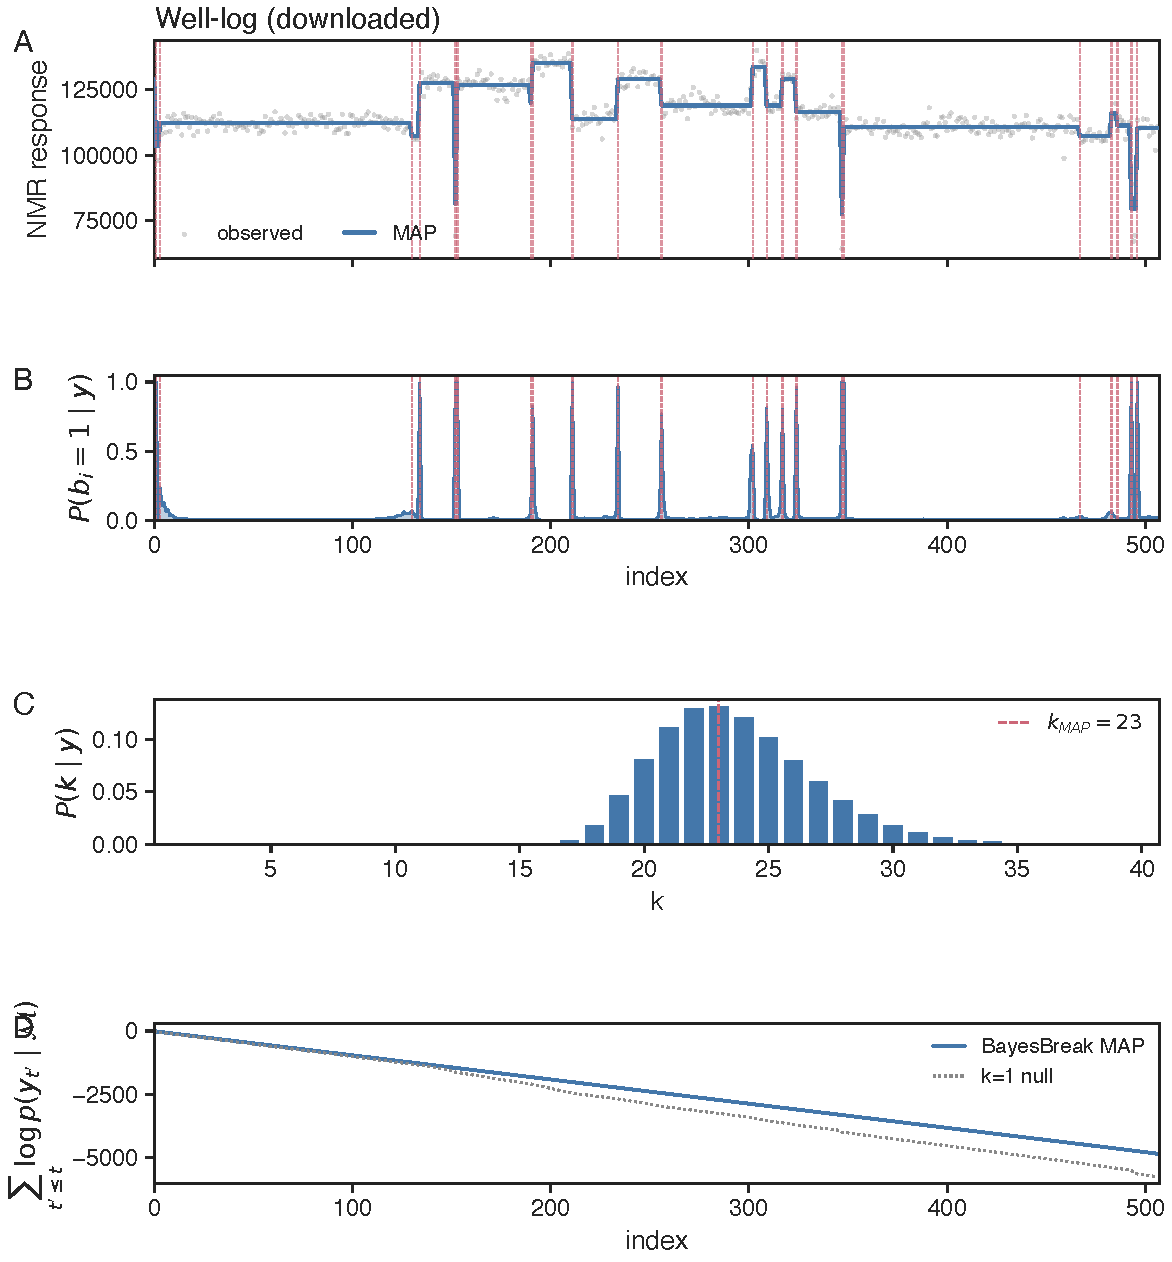
\includegraphics[width=\textwidth]{shared/figures/results/fig6_welllog.pdf}
\caption{Executed well-log fit. The solid segmentation and red vertical markers are fitted BayesBreak summaries. Boundary probabilities and $P(k\mid y)$ are posterior outputs; the cumulative panel is in-sample.}
\label{fig:welllog}
\end{figure}

\begin{table}[H]\centering\small
\begin{tabular}{@{}lrrr@{}}\toprule
Configuration & $\widehat k$ & Log evidence & Boundary entropy (nats)\\\midrule
Index-uniform, $c=h=1$ & 23 & $-4989.28$ & $36.46$\\
Archived length cohesion $c(i,j)\propto u_j-u_i$ & 25 & $-4997.15$ & $45.46$\\
\bottomrule\end{tabular}
\caption{Real archived well-log configurations. External boundary accuracy is unavailable.}
\label{tab:real_welllog}
\end{table}

The comparator cache also contains agreement-to-BayesBreak diagnostics. At tolerance three,
optimal partitioning and the Fearnhead-configured reference DP obtained agreement $F_1$ values
$0.91$ and $0.93$, respectively; binary segmentation obtained $0.86$, PELT $0.18$, and the
archived wild-binary run $0.05$. These values measure resemblance to BayesBreak's MAP boundary set,
not recovery of independently verified geology.

\subsection{Array-CGH shared boundaries}
\label{sec:realdata-cgh}
The array-CGH archive contains 43 subjects on 2,215 probes. The shared-boundary Gaussian model used
$k_{\max}=15$, returned $\widehat k=15$, and recorded pooled log evidence
$76359.79958695151$. The sum of 43 independently fitted subject evidences is
$109617.69544504143$; because the two quantities arise from different factorizations, their
difference is descriptive and is not a Bayes factor for pooling.

\begin{figure}[H]
\centering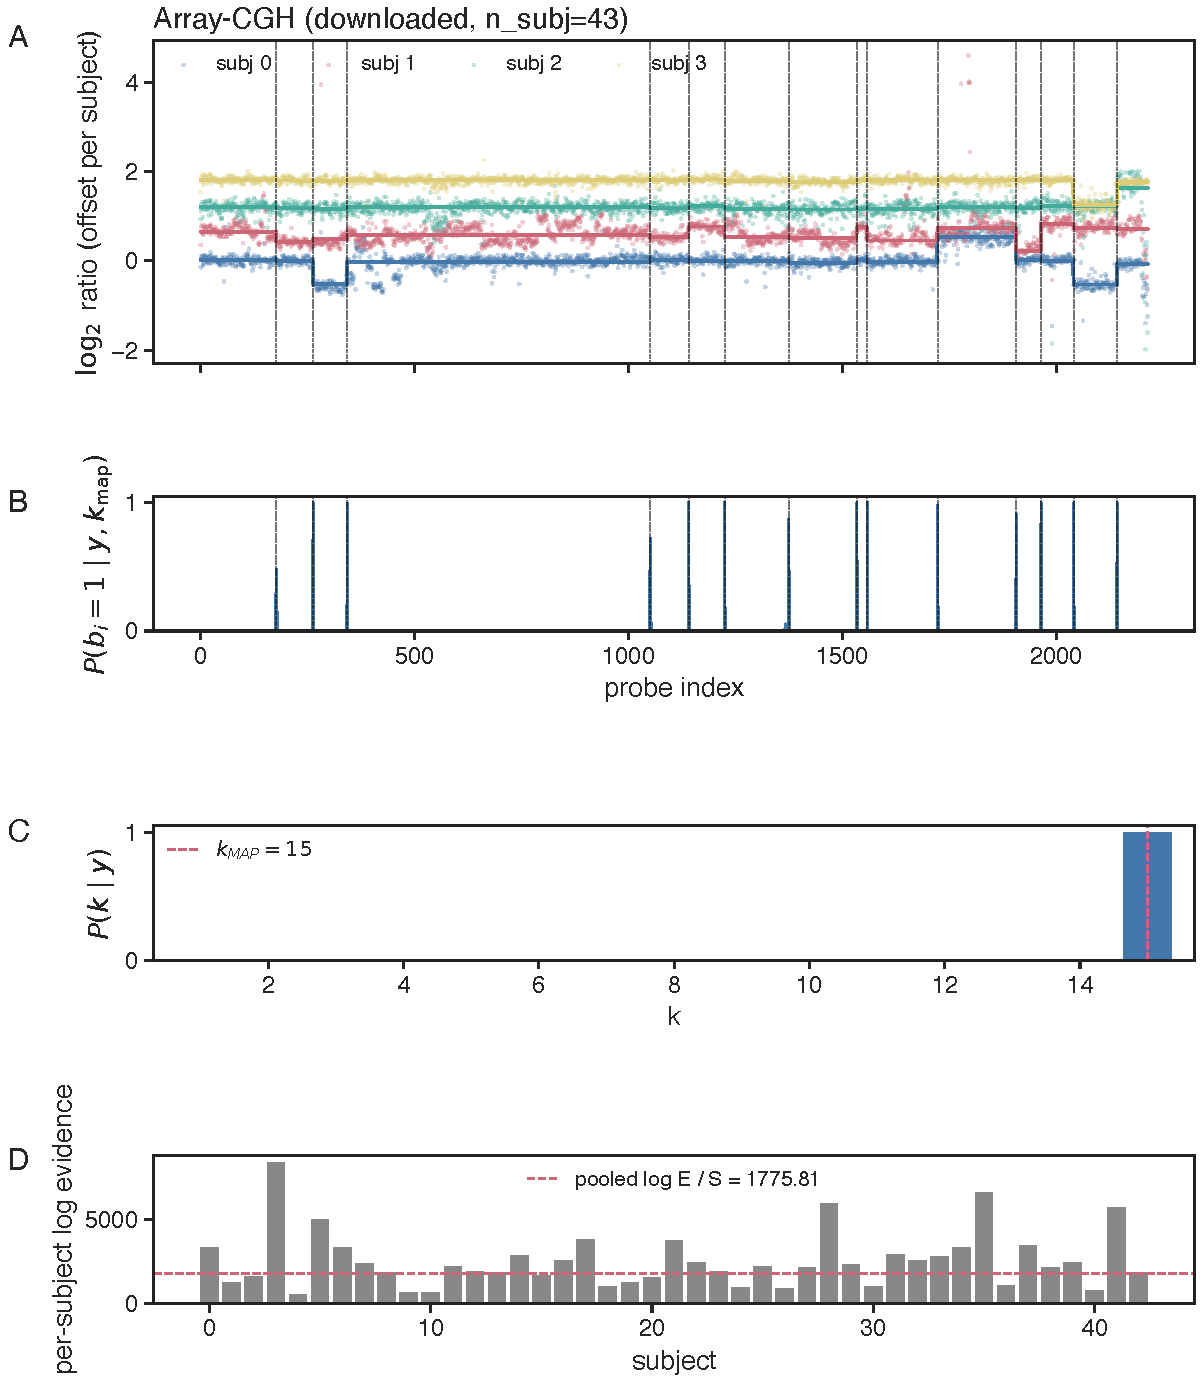
\includegraphics[width=\textwidth]{shared/figures/results/fig7_cgh.pdf}
\caption{Executed shared-boundary array-CGH fit. The common MAP segmentation is fitted across the 43-subject matrix; no external boundary annotation is asserted.}
\label{fig:cgh}
\end{figure}

\begin{exclusionbox}[RES-BB-CMP-002: incompatible comparator axis]
The comparator cache flattened a $43\times2215$ matrix into 95,245 values while retaining
BayesBreak reference boundaries on the 2,215-probe axis. The resulting zero agreement values and
large distances are real executions of an invalid comparison. They are excluded from all
scientific comparison tables. A corrected run must consume the raw subject-by-probe matrix and a
validated probe coordinate axis under a new result identifier.
\end{exclusionbox}

\subsection{S\&P 500 volatility regimes}
\label{sec:realdata-spx}
The source covers January 1, 2015 through December 31, 2023, with approximately 2,263 raw daily
observations and a stride-four executed series of $n=566$. The primary Gaussian model on
log-squared returns returned $\widehat k=29$ and log evidence $-1296.6537252802884$. The secondary
series is a Bernoulli indicator of crossing the empirical 95th-percentile threshold, not a Poisson
count; it returned $\widehat k=50$ and log evidence $-114.41004640965144$ under a different data
model, so the raw evidences are not directly comparable.

\begin{figure}[H]
\centering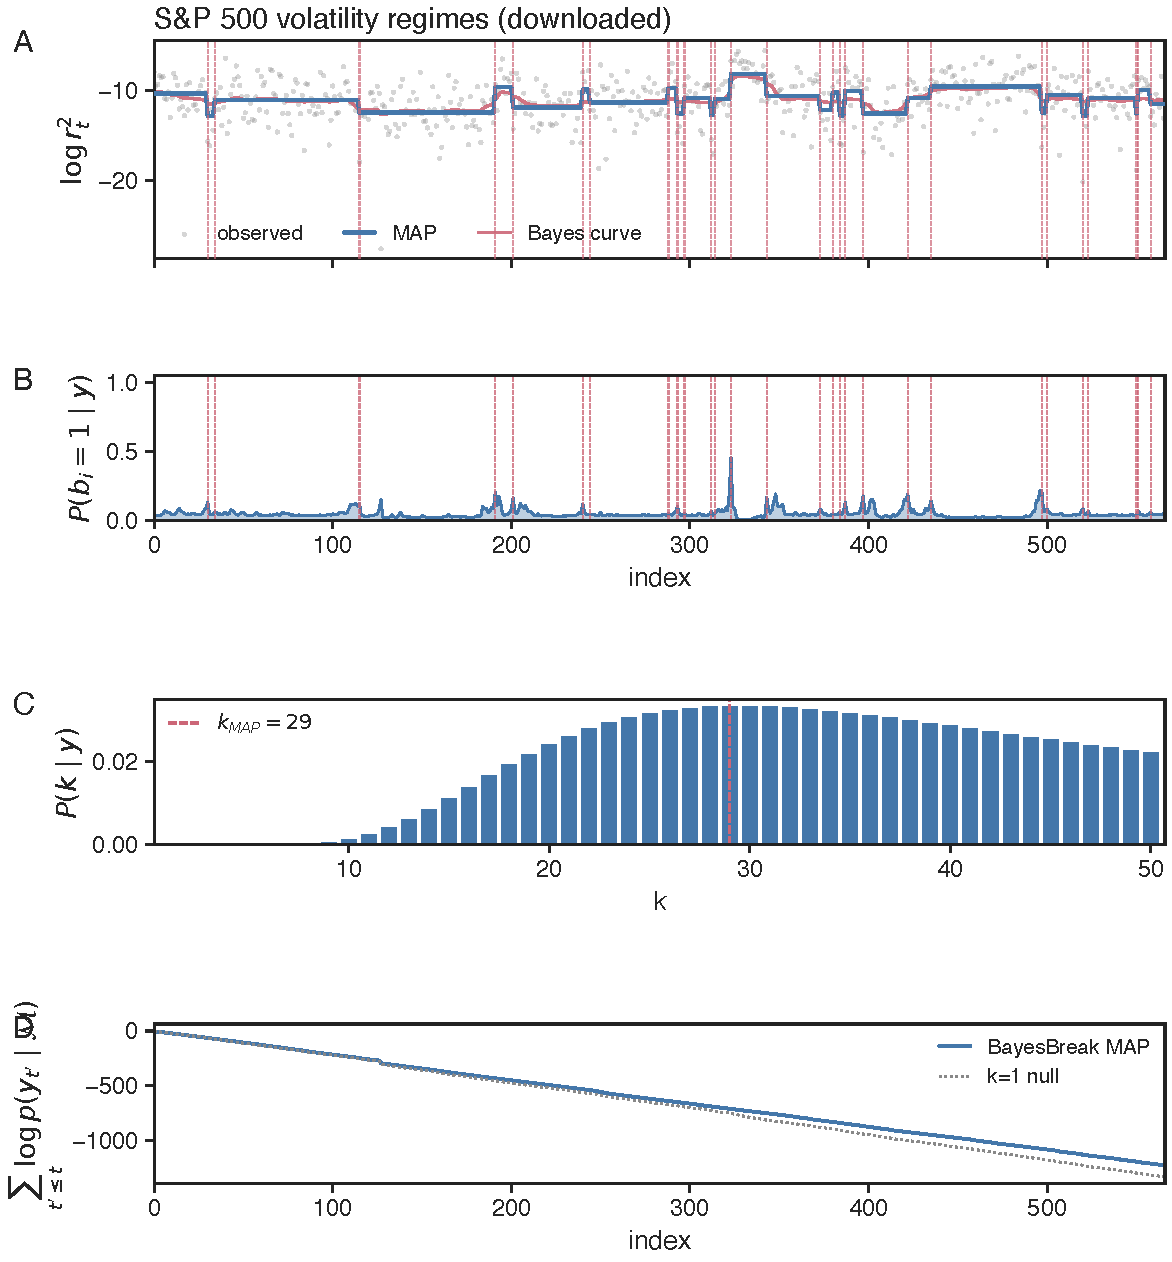
\includegraphics[width=\textwidth]{shared/figures/results/fig8_spx.pdf}
\caption{Executed S\&P 500 volatility fit for 2015--2023 after the archived stride-four preprocessing. Red markers are fitted MAP boundaries, not independently annotated macro events.}
\label{fig:spx}
\end{figure}

\begin{table}[H]\centering\small
\begin{tabular}{@{}lrrr@{}}\toprule
Method or signal & $\widehat k$ & Log evidence & Agreement $F_1@3$ vs BB Gaussian\\\midrule
BayesBreak Gaussian, $\log r_t^2$ & 29 & $-1296.65$ & reference\\
BayesBreak Bernoulli, threshold indicator & 50 & $-114.41$ & different signal\\
Optimal partitioning, matched $k$ & 29 & --- & $0.82$\\
PELT & 79 & --- & $0.53$\\
Binary segmentation, matched $k$ & 29 & --- & $0.43$\\
Wild binary segmentation, matched $k$ & 29 & --- & $0.07$\\
Fearnhead-configured reference DP & 13 & --- & $0.55$\\
\bottomrule\end{tabular}
\caption{Executed SPX outputs. Agreement columns use BayesBreak MAP boundaries as the reference and are not external accuracy.}
\label{tab:real_spx}
\end{table}

\subsection{Methylation on the methylKit chromosome-21 example}
\label{sec:realdata-methylation}
The executed data are the \texttt{methylKit} \texttt{test1.myCpG} chromosome-21 example with
$n=1904$ CpGs and per-CpG read coverage used as known precision. This is not the described Loyfer
methylation-atlas analysis. The Beta-observation quadrature fit used $k_{\max}=15$, returned
$\widehat k=15$, and recorded log evidence $-9518.667508691196$.

\begin{figure}[H]
\centering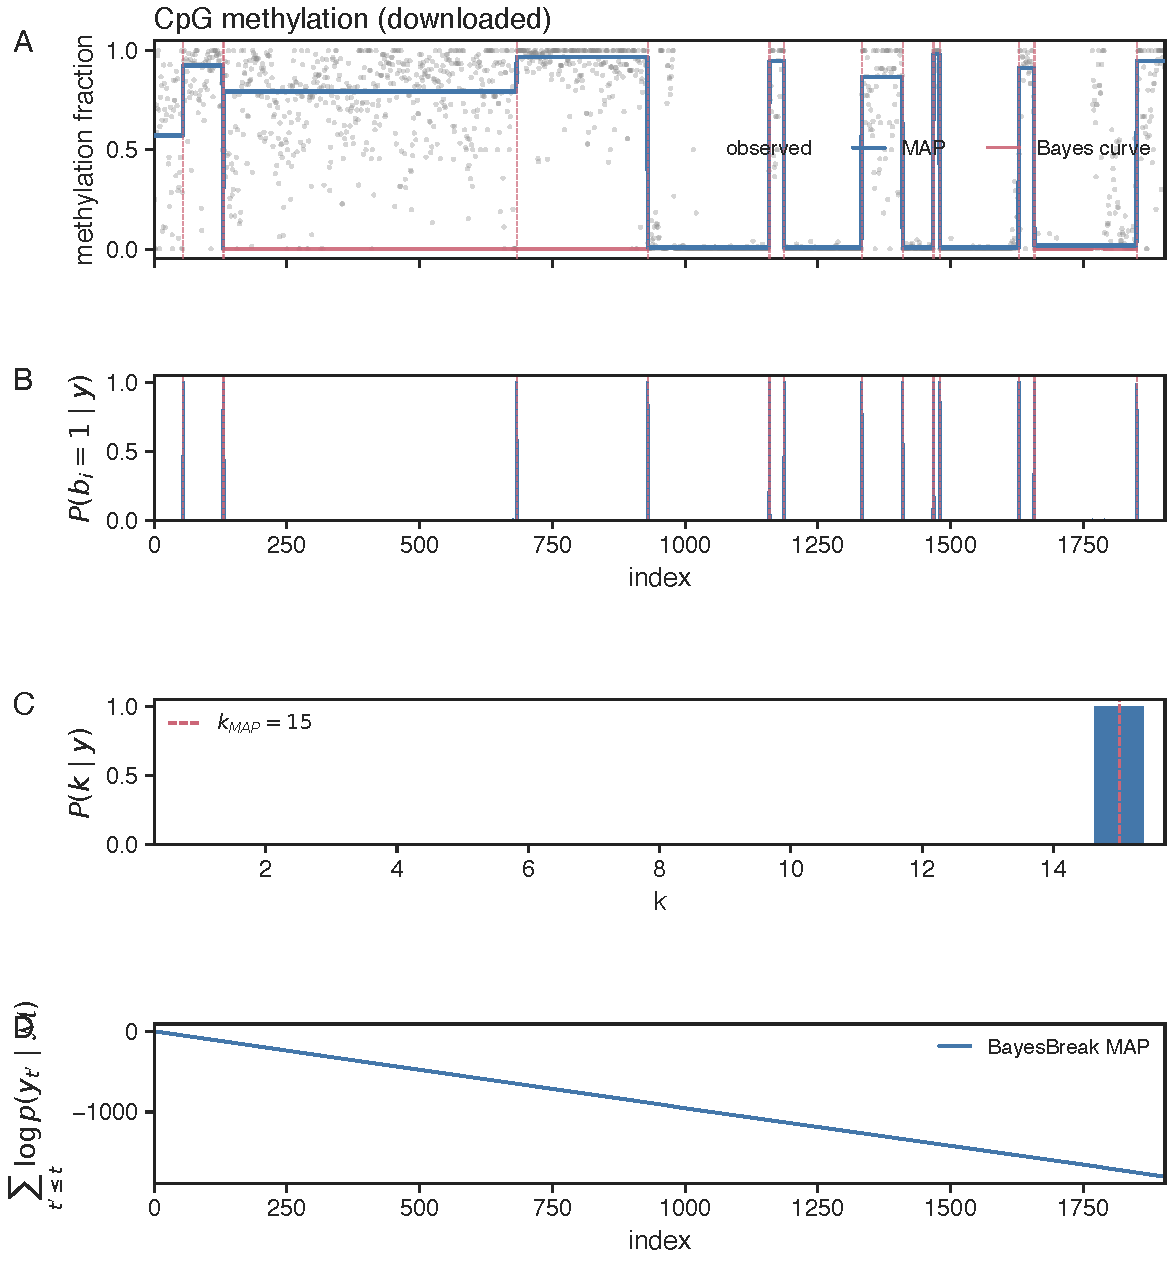
\includegraphics[width=\textwidth]{shared/figures/results/fig9_methylation.pdf}
\caption{Executed methylKit chromosome-21 Beta-observation fit. Red markers are fitted MAP boundaries; no atlas transition annotation is present in the archived source.}
\label{fig:methylation}
\end{figure}

\begin{table}[H]\centering\small
\begin{tabular}{@{}lrrr@{}}\toprule
Method & $\widehat k$ & Runtime (s) & Agreement $F_1@3$ vs BB\\\midrule
BayesBreak Beta-observation & 15 & --- & reference\\
Optimal partitioning, matched $k$ & 15 & $46.89$ & $0.79$\\
Binary segmentation, matched $k$ & 15 & $0.10$ & $0.57$\\
PELT & 5 & $3.32$ & $0.44$\\
Wild binary segmentation, matched $k$ & 15 & $0.76$ & $0.14$\\
\bottomrule\end{tabular}
\caption{Executed methylation comparator agreement. No external atlas accuracy is claimed.}
\label{tab:real_methylation}
\end{table}

\begin{exclusionbox}[RES-BB-RD-007Q: invalid family/support predictive path]
The archived held-out value $-387.50040013308154$ for $m=381$ remains in the result ledger. It is
not shown as valid held-out performance because the implementation used a Gaussian fallback for a
Beta-observation estimator and silently clipped out-of-range coordinates to the last MAP block.
The segmentation fit and its log evidence remain admissible descriptive real results.
\end{exclusionbox}

\section{What these case studies establish}
Together, the fits demonstrate that the implemented interface executed on Gaussian single-series,
Gaussian shared-boundary, Gaussian volatility, Bernoulli threshold, and Beta-observation settings,
and that their archived DP invariants passed. They do not establish external boundary accuracy,
causal correspondence to domain events, or superiority to comparators. Those claims require the
predeclared protocols in Appendix~\ref{app:experiments}.
